\section{Modifying and applying RISE (Single Pixel)}
\nblink{brats/06\_rise.ipynb}

apply on a single pixel, pixel == class

\subsection{Results}

\begin{figure}[H]
\centering
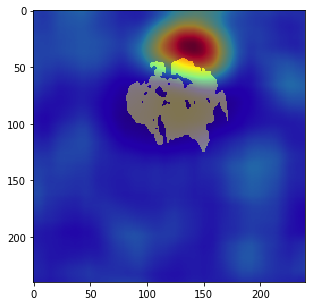
\includegraphics[width=8cm]{chapters/04_segmentation/images/rise_single_pixel.png}
\caption{Saliency map analyzing the topmost pixel in the scan, overlaid on the generated network output}
\end{figure}



\subsection{Discussion}
looks correct, maybe a bit off => could be scaling

The produced output looks correct, the color blob is at the correct position. It clearly shows that the neural network looks at the correct location to generate the segmentation.
Apart from this basic correctness verification, no further insigt is provided by the saliency map, because the resolution generated by RISE is too low.

\subsection{Conclusion}
The generated output is low resolution but still helpful, we therefore decided to build a version of RISE which works on all pixels of the segmentation.

\section{Modifying and applying RISE (Multi Pixel)}
\nblink{17\_rise\_multipixel.ipynb}

TODO: implementation

\subsection{Results}
\begin{figure}[H]
    \centering
    \begin{subfigure}{.5\textwidth}
        \centering
        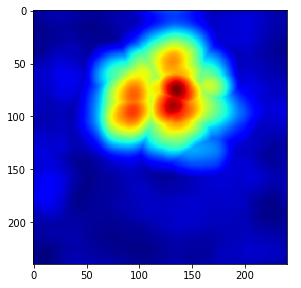
\includegraphics[width=\linewidth]{chapters/04_segmentation/images/rise_multipixel_max_1-0.png}
        \caption{ the text for a}
    \end{subfigure}%
    \begin{subfigure}{.5\textwidth}
        \centering
        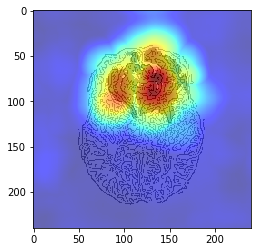
\includegraphics[width=\linewidth]{chapters/04_segmentation/images/rise_multipixel_max_1-1.png}
        \caption{b}
    \end{subfigure}
    \caption{Explanation text}
\end{figure}

\subsection{Discussion}

\subsection{Conclusion}
